\graphicspath{{mehul_pics/}}% Set graphics path location

%\subsection{Additional Test Image Results}
\subsubsection{Test Image Results: Blurry Friends}

\begin{figure}[H]
        \centering
        \begin{subfigure}[b]{0.49\textwidth}
                \centering
                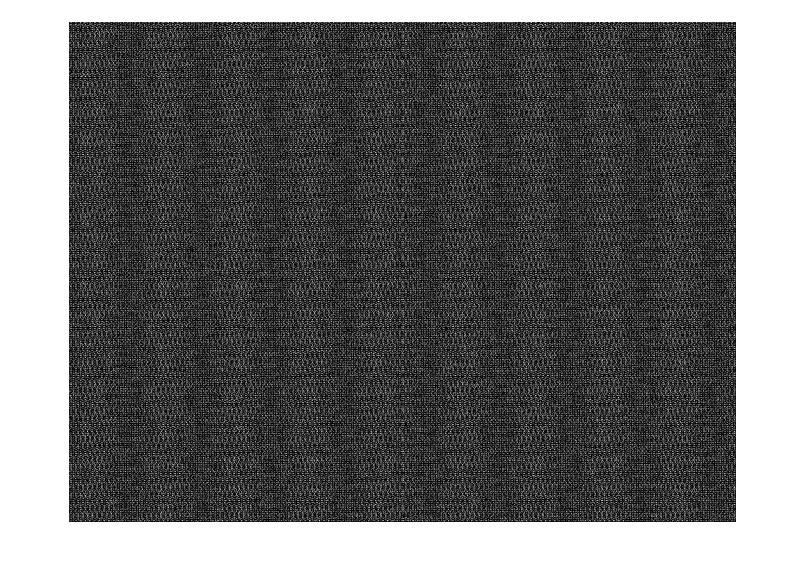
\includegraphics[width=\textwidth]{inverse.jpg}
                \caption{Using Inverse Filter.}
        \end{subfigure}
        \begin{subfigure}[b]{0.49\textwidth}
                 \centering
                 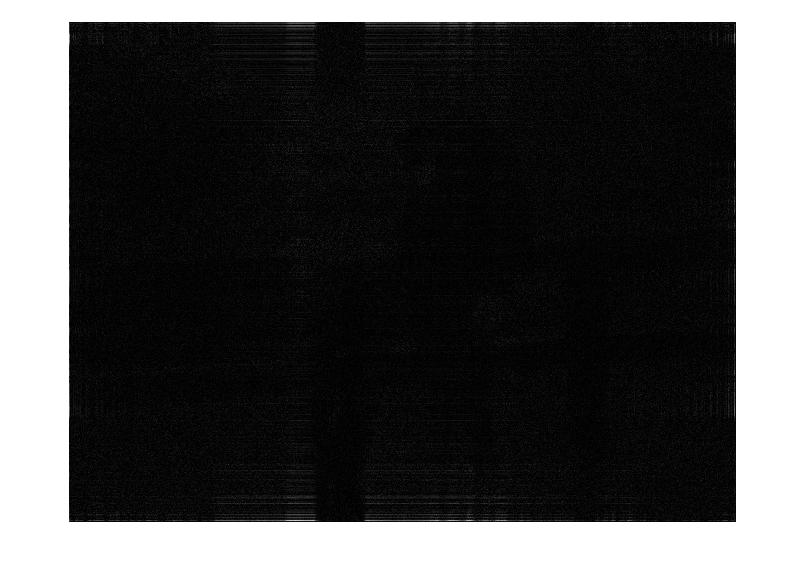
\includegraphics[width=\textwidth]{pseudo_inverse.jpg}
                 \caption{Using Pseudo Inverse Filter.}
                 \label{fig:friends}
                       
        \end{subfigure}             
        \caption{Real blurry image sharpening using Inverse and Pseudo Inverse filters} 
\end{figure}

\begin{figure}[H]
        \centering
        \begin{subfigure}[b]{0.49\textwidth}
                \centering
                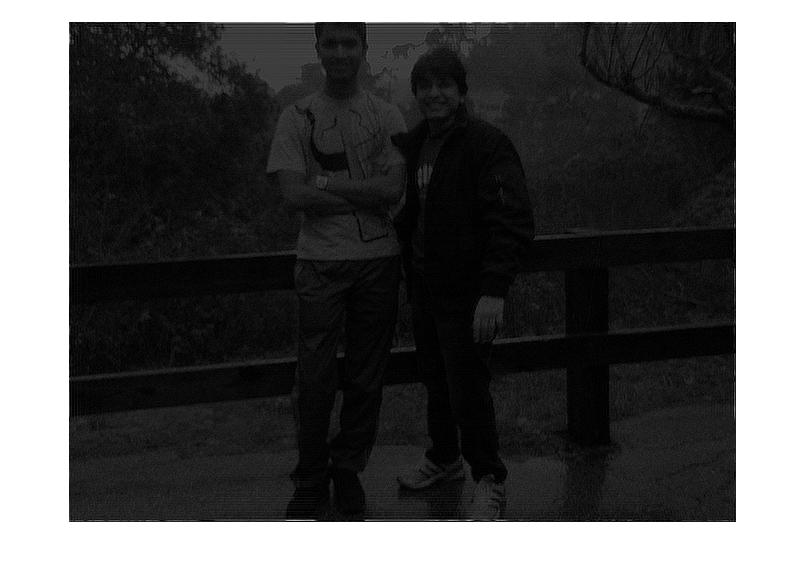
\includegraphics[width=\textwidth]{geo_mean.jpg}
                \caption{Using Geometric Mean Filter.}
        \end{subfigure}
        \begin{subfigure}[b]{0.49\textwidth}
                 \centering
                 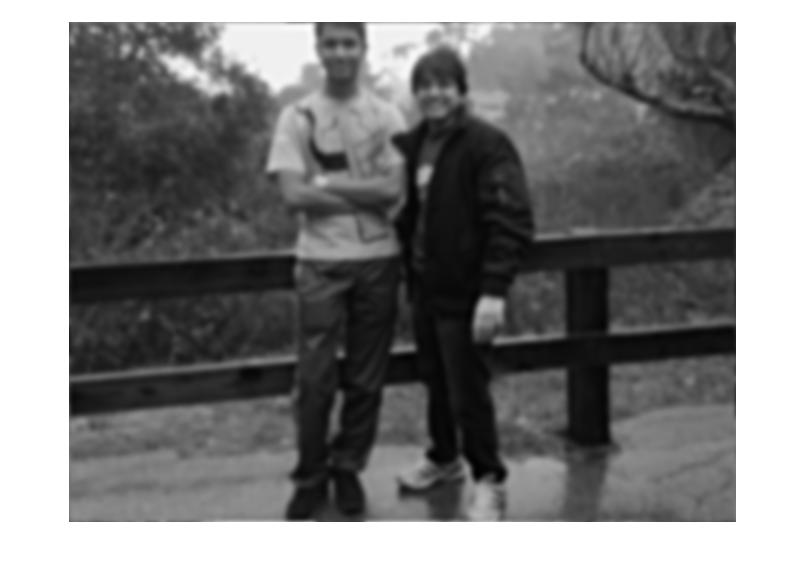
\includegraphics[width=\textwidth]{least_squares.jpg}
                 \caption{Using Least squares Filter.}
                 \label{fig:friends}
                       
        \end{subfigure}             
        \caption{Real blurry image sharpening using Geometric mean and least squares filters}
\end{figure}

Restored Image sharpness order,
\begin{equation*}
Wiener > Geometric~Mean > Constrained~Least~Squares > Pseudo~Inverse~Filter > Inverse Filter
\end{equation*}
\noindent Geometric Mean filter does the best (after Wiener) among these filters in recovering a sharp image. The magnitude of inherent noise in the test image corrupts images retrieved when using Inverse and Pseudo Inverse filters.
\newpage